\section{Softwarearchitektur} \label{sec:Softwarearchitektur}

\todoin{Beschreibung der Schnittstellen, z.B. Dateien und ihre Struktur, Benutzte Module/Bausteine und ihre Einbindung, Installationsvorschriften}

Die Software des Spiels "'Schiffe versenken"' wurde als Client-Server Anwendung gemäß Abbildung \ref{fig:Kommunikationsteilnehmer} entworfen.
Die zentrale Kommunikationsschnittstelle stellt der Kommunikationsserver dar, der auf dem Port $54321$ eingehende Verbindungen annimmt.
Verbindungen können sowohl mittels eines Java-Clients hergestellt werden, die von einem Menschen bedient werden, als auch von Prolog-Clients, die vollständig autonom agieren.
Es liegen hinsichtlich der Clientkombinationen keine Beschränkungen vor, sodass auch z.B. ein Prolog-Client gegen einen anderen Prolog-Client antreten kann.

\begin{figure}[H]
  \centering
  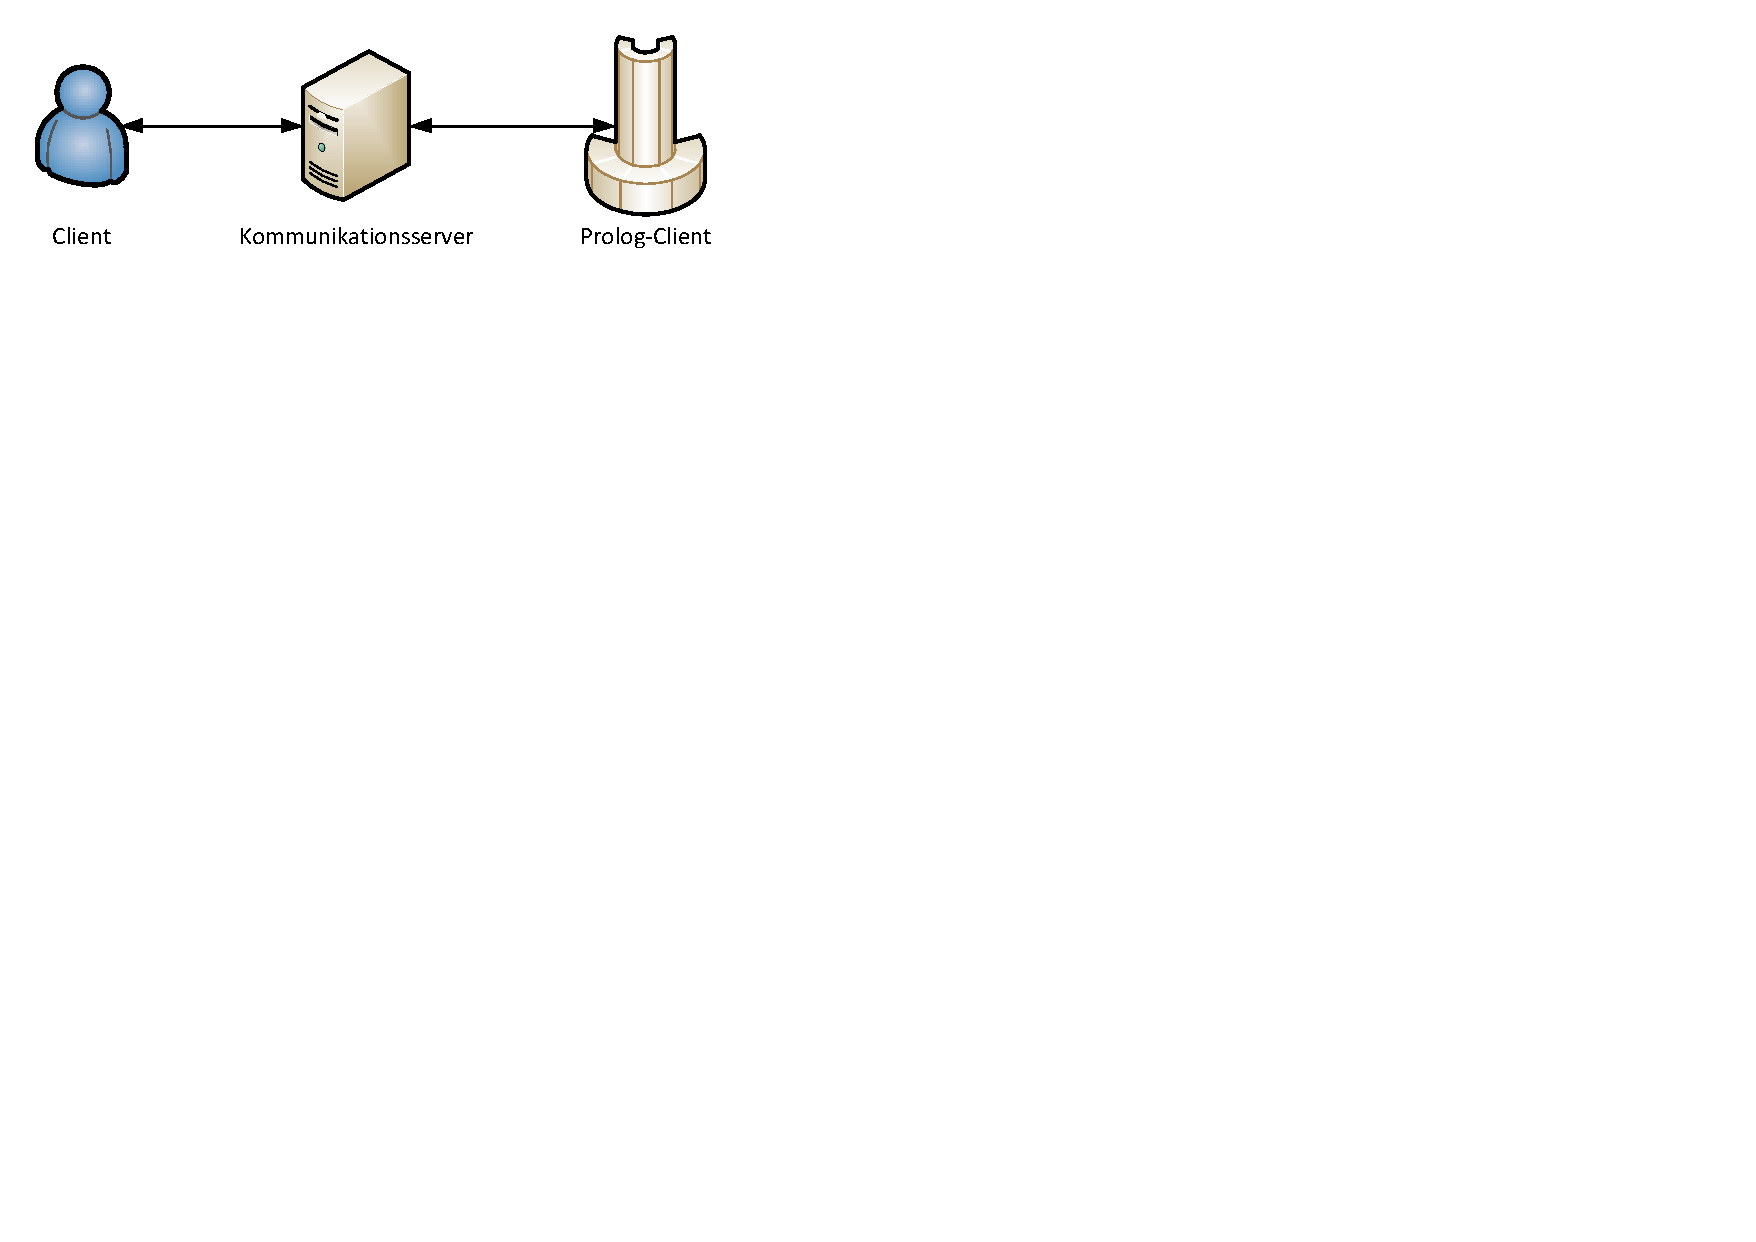
\includegraphics[trim=0mm 165mm 175mm 0mm,clip,width=0.5\textwidth]{images/Kommunikationsmodell.pdf}
  \caption{Darstellung der möglichen Kommunikationsteilnehmer}
  \label{fig:Kommunikationsteilnehmer}
\end{figure}

Der gesamte Spielverlauf lässt sich anhand der Statusdiagramme in den Abbildungen \ref{fig:Clientstates} und \ref{fig:SubClientstates} beschreiben.
Diese sind sowohl für den Javaclient, als auch für das Prologprogramm gültig.

Unmittelbar nach Start des Clients befindet sich dieser im Initialisierungszustand \emph{INITIALIZATION}.
Während dieser Phase obliegt es dem Client seine Schiffe gemäß den Regeln zu platzieren.
Des Weiteren hat er eine Nachricht des Servers zu empfangen, die angibt, ob sein initialer Zustand \emph{DEFENCE} oder \emph{ATTACK} sein soll, wenn er in die \emph{RUNNING}-Phase übergeht.
Dieser Übergang erfolgt durch den Empfang des Startkommandos, mit dem Opcode = 5.

\begin{figure}[H]
  \centering
  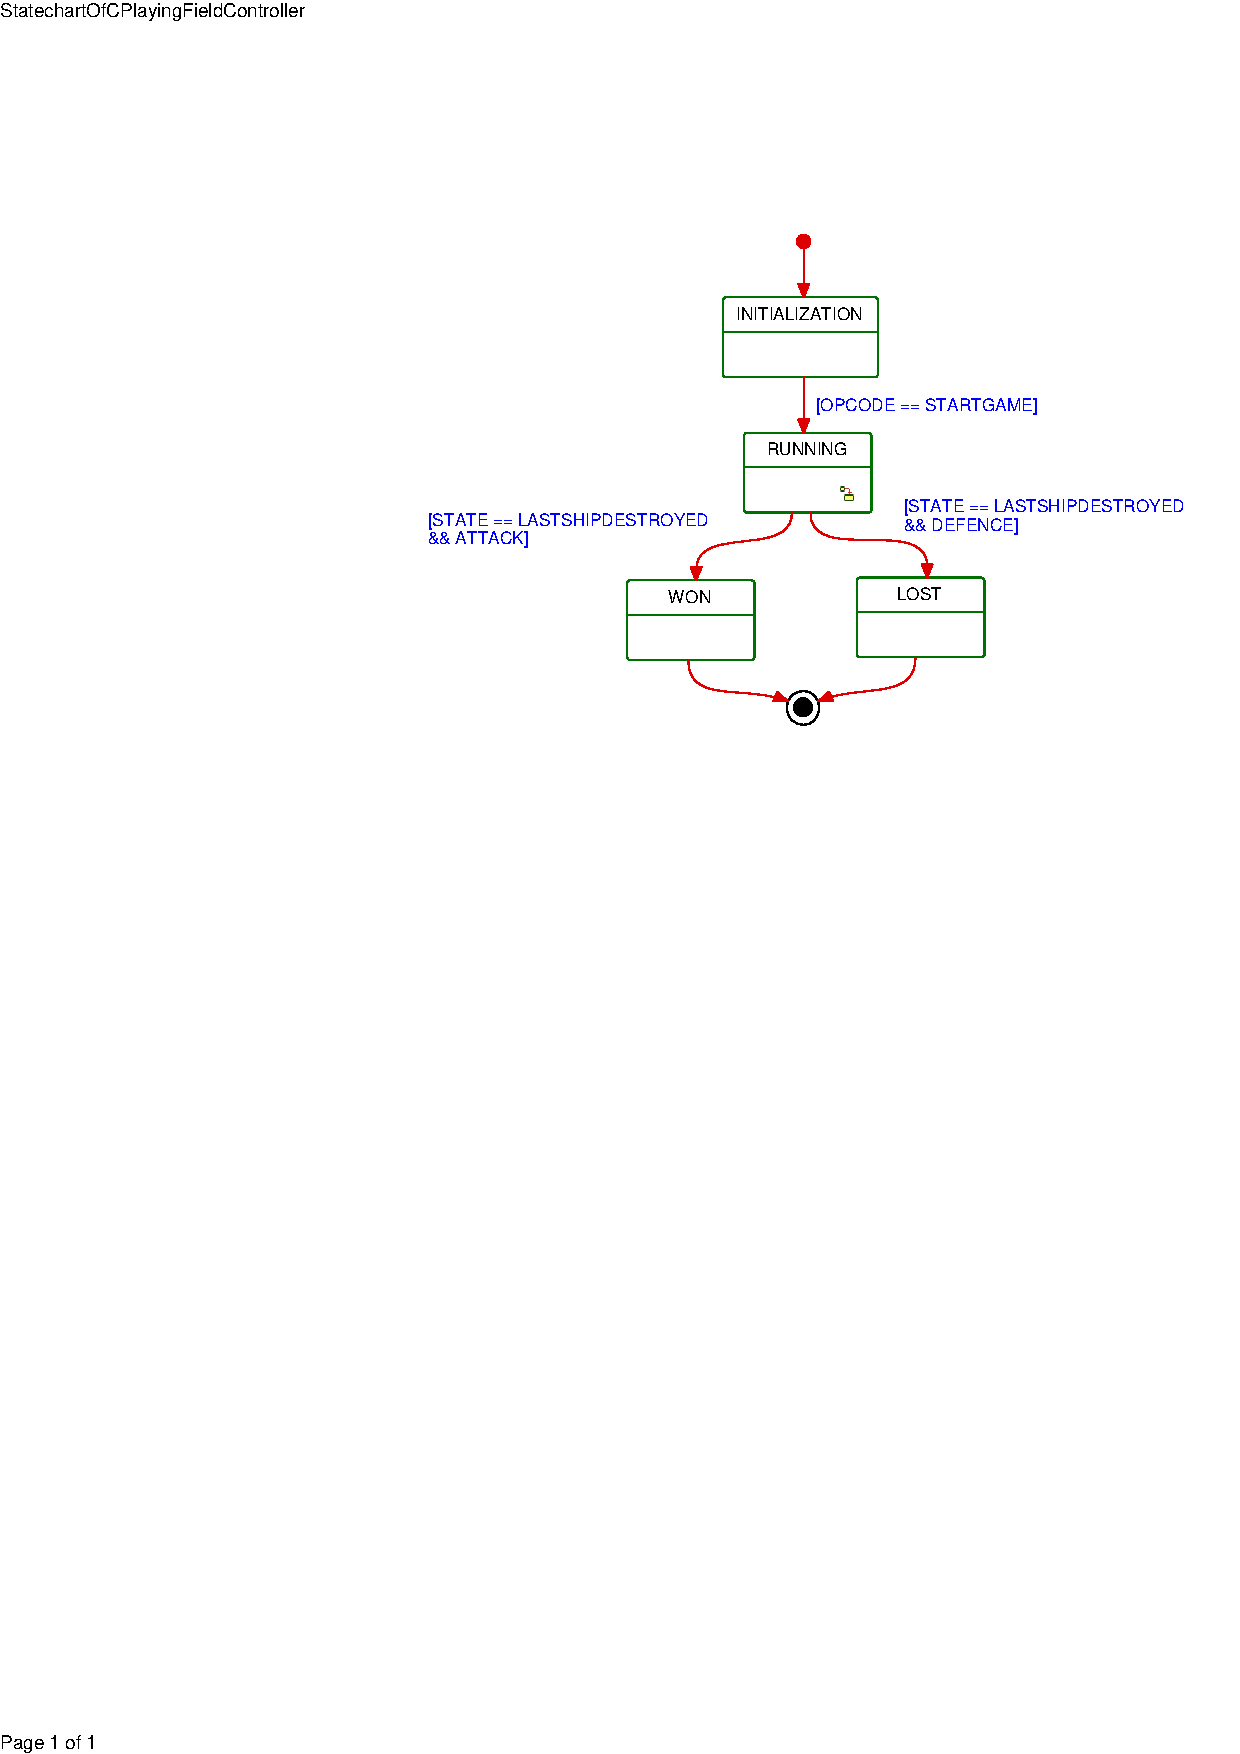
\includegraphics[trim=70mm 170mm 5mm 39mm,clip,width=0.7\textwidth]{images/SMController.pdf}
  \caption{Zustandsübergänge des Clients}
  \label{fig:Clientstates}
\end{figure}

%\todoin{Vic - Bemerkung zur Grafik: es gibt doch garkeinen OPCODE == LOST oder WON? Meiner Meinung nach wird der Zustandsübergang wird durch 'letztes Schiff versenkt' ausgelöst und dann hängt es davon ab, ob es das eigene ist oder nicht..? gleiches gilt für die folgende abbildung}

Befindet sich der Client im \emph{RUNNING}-Status, so wechselt er zwischen seinen internen Zuständen \emph{ATTACK} und \emph{DEFENCE} hin und her.
Dieser Wechsel erfolgt immer dann, wenn eine \emph{ATTACKRESPONSE} Nachricht mit dem Opcode = 2 übertragen wurde.
Der primäre Unterschied zwischen beiden Zuständen ist die Reihenfolge der erwarteten Nachrichten.
Befindet sich der Client im Subzustand \emph{DEFENCE}, so erwartet er von seinem Kontrahenten eine Nachricht mit dem Opcode = 1 und beantwortet diese seinerseits mit dem Opcode = 2.
Sollte sich der Client im Subzustand \emph{ATTACK} befinden, so sendet er zuerst die Nachricht mit dem Opcode = 1 und erwartet im Anschluss eine Nachricht seines Gegners.

Das Alternieren der Zustände erfolgt solange, bis in der Antwortnachricht mit dem Opcode = 2 eine Meldung über den Verlust aller Schiffe transferiert wird.
Dieses Ereignis wird gemäß Tabelle \ref{tbl:Ergebniskodierung} auf Seite \pageref{tbl:Ergebniskodierung} mit dem Ergebniscode = 4 beschrieben.
Empfängt der Client die Nachricht, so gilt das Spiel als gewonnen.
Umgekehrt verliert der Client das Spiel, wenn er diese Nachricht verschickt.

Im Rahmen dieses Kontexts wechselt der Spielzustand in \emph{WON} bzw. \emph{LOST} und das Programm kann beendet werden.

\begin{figure}[H]
  \centering
  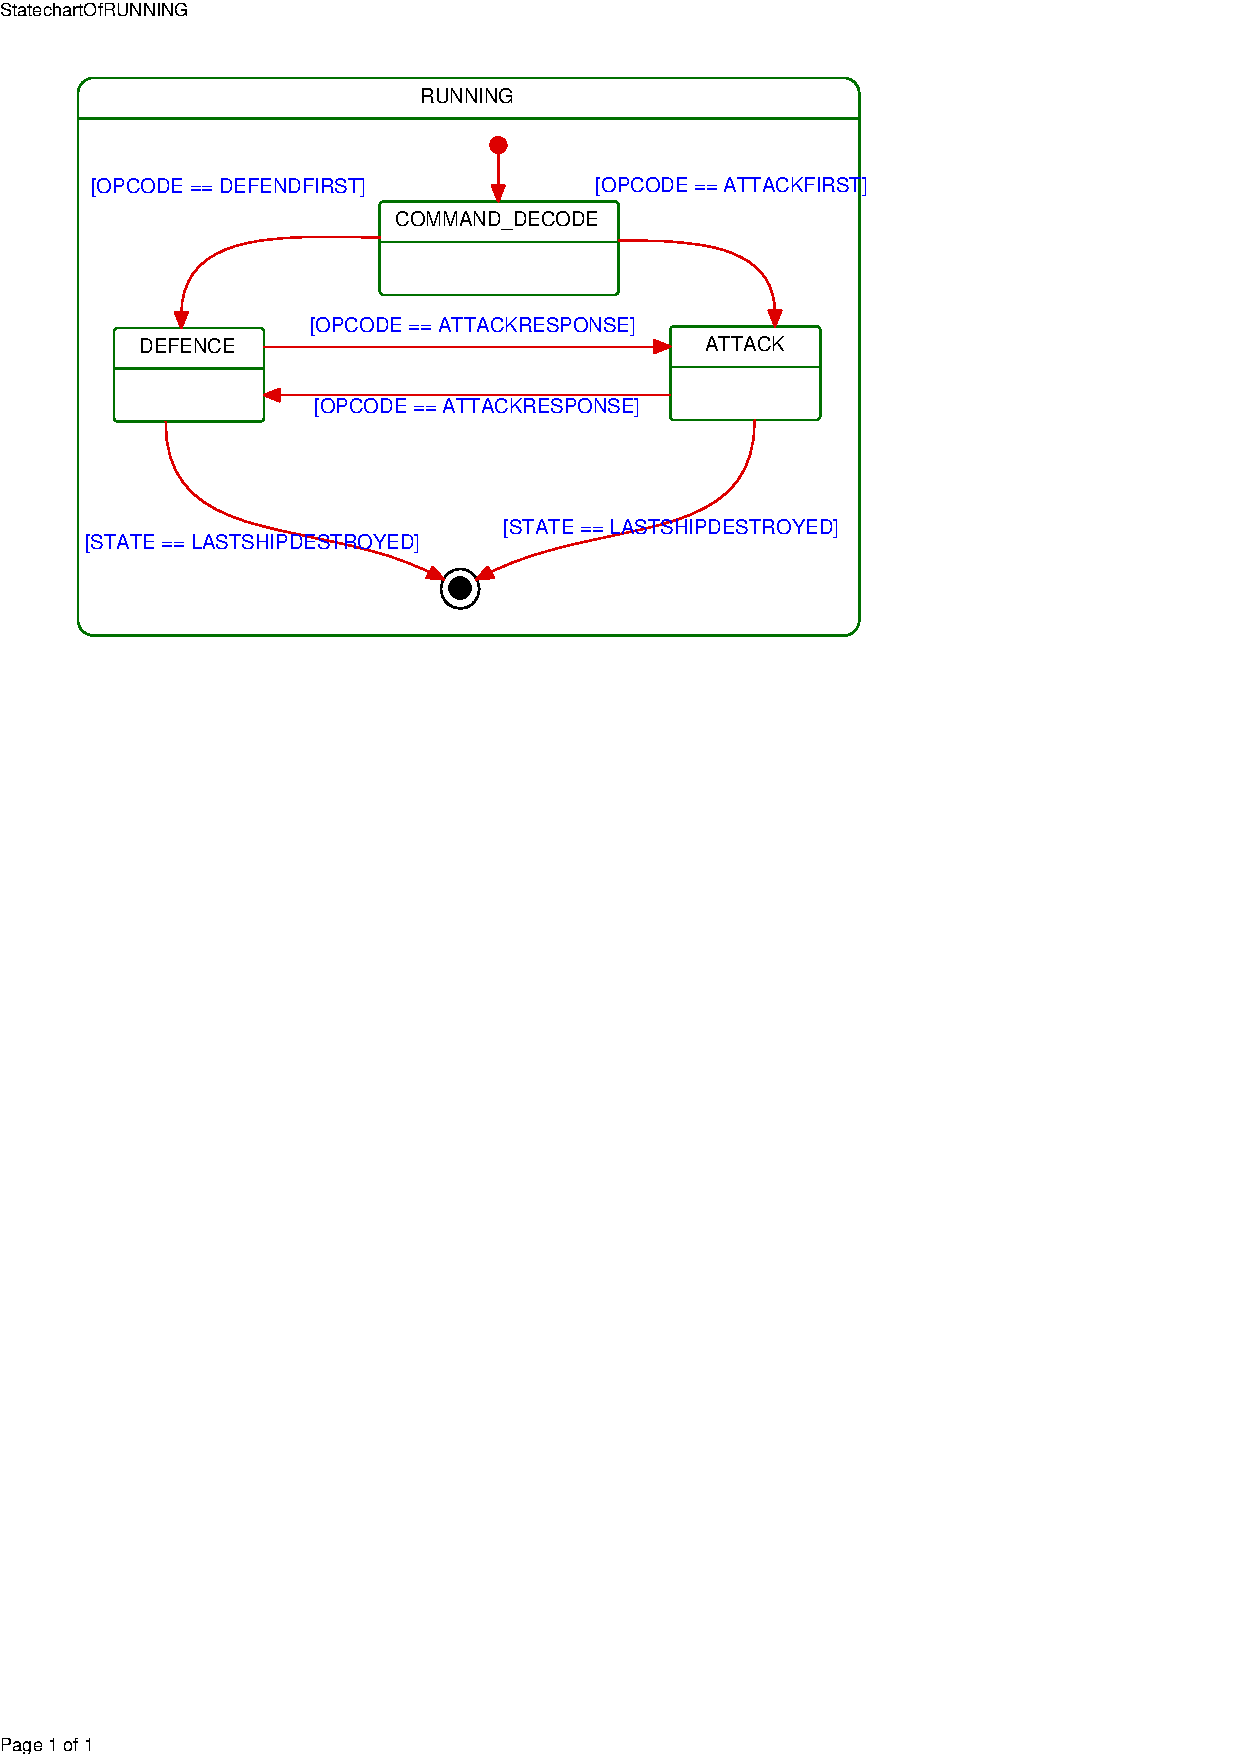
\includegraphics[trim=10mm 185mm 60mm 10mm,clip,width=0.5\textwidth]{images/SubSMRUNNING.pdf}
  \caption{Interne Zustandsübergänge während des laufenden Spiels}
  \label{fig:SubClientstates}
\end{figure}

Die vorgesehene Kommunikationsabfolge wird ebenfalls in Abbildung \ref{fig:Kommunikationssequenz} in Form eines Sequenzdiagramms dargestellt.
Das Diagramm stellt einen beispielhaften Spielablauf mit einem Prolog-Client und einem Java-Client dar. 
Der Client, der sich zuerst mit dem Server verbindet, beginnt per Konvention im Verteidungsmodus und der zweite verbundene Client startet im Angriffsmodus.
Erst wenn sich zwei Teilnehmer am Server verbunden haben, sendet dieser das Startsignal an alle Clients.

Die Spielphase wird durch eine Schleife bestimmt, in der die Teilnehmer von den Angriffs- in den Verteidigungszustand wechseln und umgekehrt.
Die dabei übertragenen Nachrichten werden stets an den Server übertragen, der diese an den jeweils anderen Client weiterleitet.
Dadurch kommt keine direkte Verbindung beider Spieler zustande.

Das Programmende aus Sicht der Kommunikation wird erreicht, wenn ein Spieler die Nachricht überträgt, dass er über keine Schiffe mehr verfügt.
In diesem Fall werden die Verbindungen getrennt und der Server kann neue Verbindungen von Spielern zum Ausrichten eines neuen Spiels annehmen.

\begin{figure}[H]
  \centering
  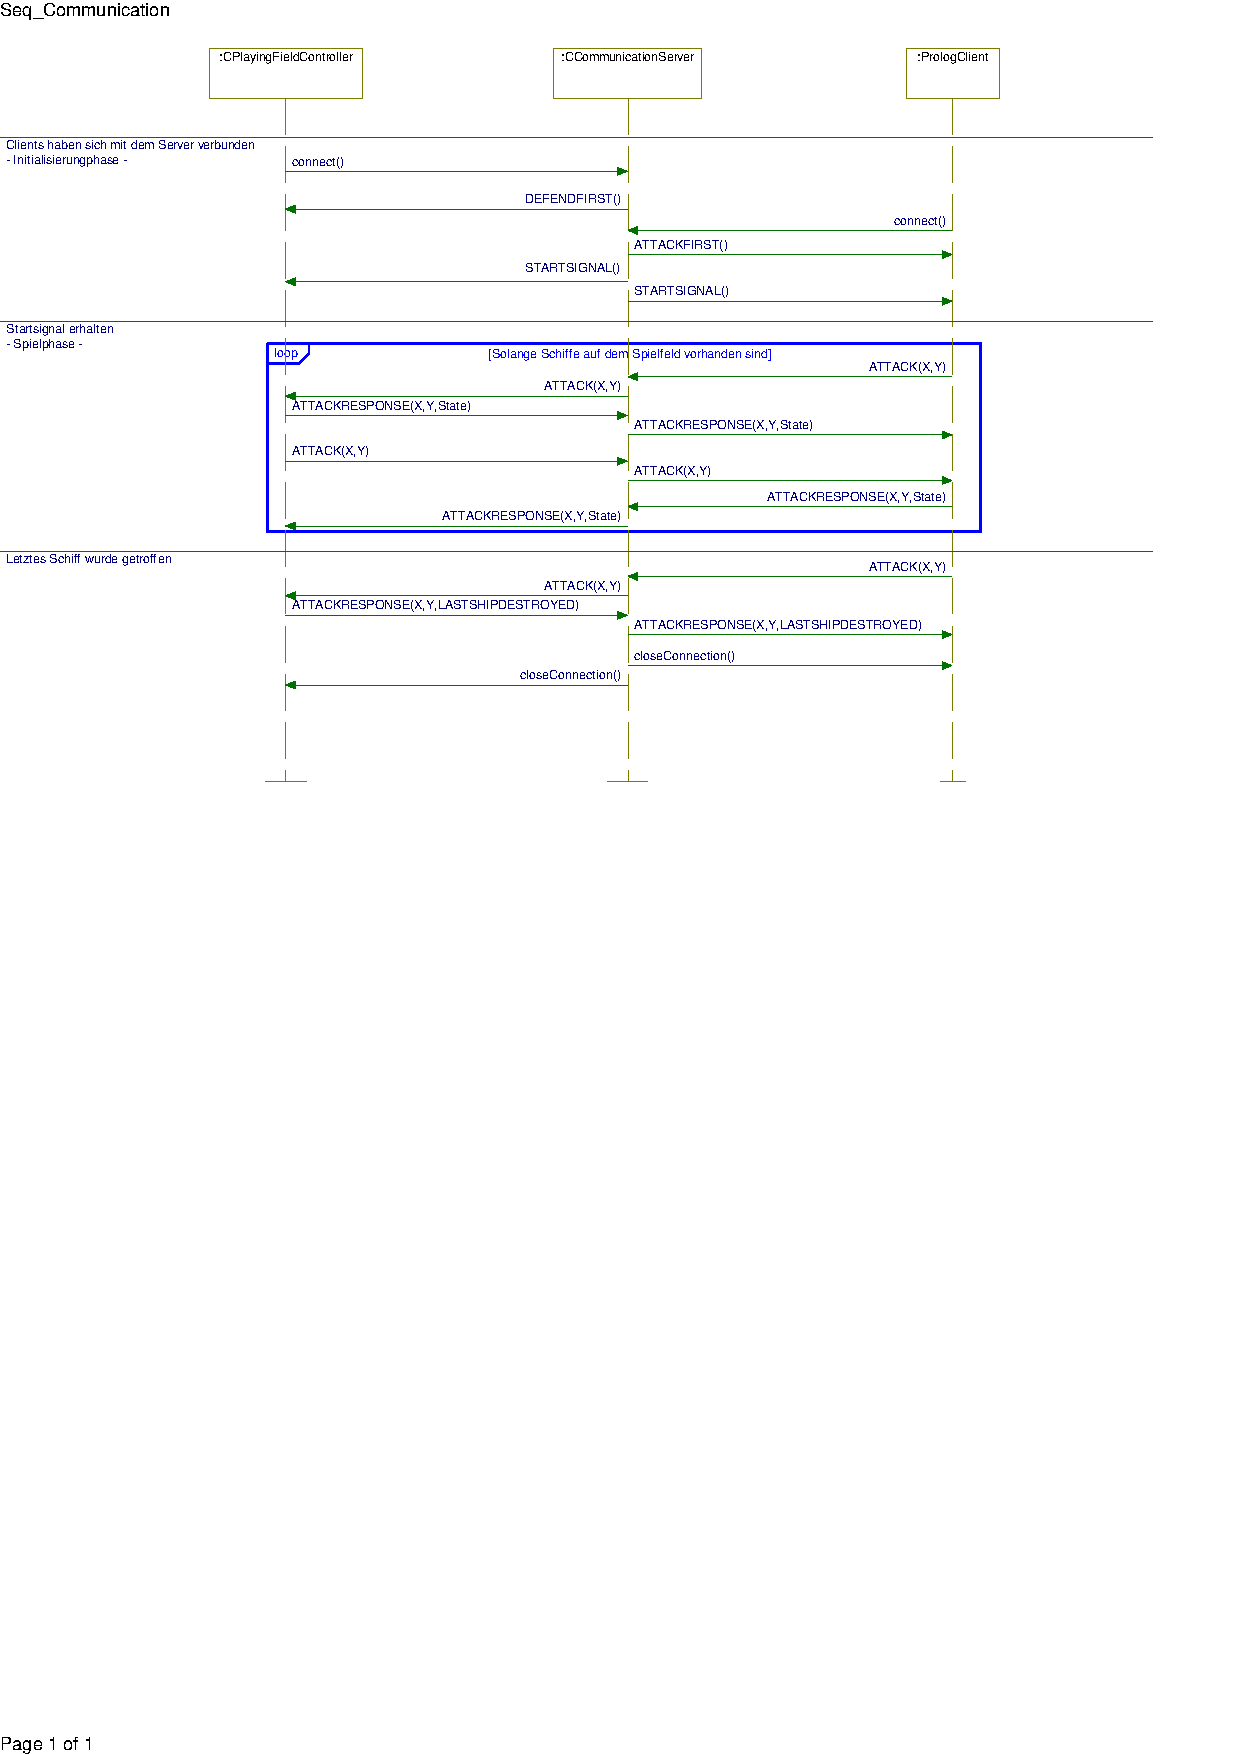
\includegraphics[trim=0mm 160mm 25mm 5mm,clip,width=0.95\textwidth]{images/SeqCommunication.pdf}
  \caption{Sequenzdiagramm der Kommunikation}
  \label{fig:Kommunikationssequenz}
\end{figure}

